%****************************************************
%	CHAPTER 3 - Dynamics
%****************************************************
\chapter{Kinematics \& Dynamics}
\label{ch:dynamics}
%====================================================
Generally applicable rigid body dynamics are first derived with respect to net forces and torques. Thereafter, those dynamics are adapted to the non-linear multibody case where constrained relative rotational motion between bodies in permitted. Following that, aerodynamic effects incorporated into the plant's model. Finally a consolidated, quaternion based plant model is presented which is used for the later control plant development next in Chapter:\ref{ch:control}.
%====================================================
\section{Rigid Body Dynamics}
\label{sec:dynamics.rigidbody}
%====================================================
\subsection{Lagrange Derivation}
\label{subsec:dynamics.rigidbody.lagrange}
%====================================================
Fundamentally any body, rigid or otherwise, can undergo two kinds of movements, namely rotational and translation motions. Often a Lagrangian\cite{classicaldynamics,rotationrigidbody} approach for combined angular and translational movements is used to derive the differential equations of motion for each degree of freedom. The Lagrangian principle ensures that (translational and rotational) kinematic energies and potential energy are conserved throughout the system's trajectory progression. When combined with Euler-Rotational equations, the Euler-Lagrangian\cite{lagrange-formalism} formulation fully defines the aerospace 6-DOF equation set.
\par
Lagrangian formalism is regarded as especially useful in non-cartesian (\emph{spherical etc\ldots}) co-ordinate frames or multi-body systems. With that being said, a cartesian co-ordinate system was already defined in Sec:\ref{subsec:proto.conventions.motoraxis}. Rigid body dynamics in a cartesian co-ordinate frame do lend themselves to Newtonian mechanics. The Newton-Euler or Euler-Lagrange formulations both stipulate the same resultant differential equations of motion. The Lagrangian operator, $\mathcal{L}$, is a term consisting of the difference between kinetic and potential energies, $T$ and $U$ respectively. Considering some generalized path co-ordinates $\mathbf{r}(t)$, for both position $\vec{\mathcal{E}}$ and attitude $\vec{\eta}$ relative co-ordinates;
\begin{equation}\label{eq:generalpath}
\mathbf{r}(t)=\begin{bmatrix}
\vec{\mathcal{E}}\hspace{3pt}\\
\vec{\eta}
\end{bmatrix}
\end{equation}
The co-ordinates in Eq:\ref{eq:generalpath} are generalized here, despite being symbols commonly used to represent linear and attitude positions. The generalized co-ordinates are later be refined to Cartesian body co-ordinates with respect to the inertial frame. The Lagrangian is, by definition:
\begin{subequations}
\begin{equation}\label{eq:lagrangian.a}
\mathcal{L}(\mathbf{r},\dot{\mathbf{r}},t)=T(\mathbf{r},\dot{\mathbf{r}})-U(\mathbf{r},\dot{\mathbf{r}})
\end{equation}
With kinetic and potential energy function(s) $T$ and $U$ respectively. Then introducing a rigid body's general (linear \& angular) kinetic and potential energies, in some shared reference frame $\mathcal{F}^x$. 
\newpage
In this case the only potential energy is gravitational\footnote{Here gravity is defined as; $G=\begin{bmatrix}
0&0&-9.81
\end{bmatrix}^T~m.s^{-2}$~in the Inertial frame,$\in\mathcal{F}^I$} potential energy:
\begin{equation}\label{eq:lagrangian.b}
\mathcal{L}=
\frac{1}{2}
\begin{bmatrix}
\dot{\vec{\mathcal{E}}}^{~T}(m)\dot{\vec{\mathcal{E}}}\\
\dot{\vec{\eta}}^{~T}(\mathbb{I}_b)\dot{\vec{\eta}}
\end{bmatrix}
-
\begin{bmatrix}
m\vec{G}z\\
0
\end{bmatrix}
\end{equation}
\end{subequations}
Noting that $\mathbb{I}_b$ is the inertial tensor of the body aligned and translated w.r.t whichever reference frame is used. The Euler-Lagrange formulation equates partial derivatives of the Lagrangian to any generalized forces, $\mathbf{V}$, acting on the system. In this case the generalized forces are, more specifically, a net force $\vec{F}_{net}$ and a net torque $\vec{\tau}_{net}$.
\begin{equation}\label{eq:euler-lagrange}
\frac{d}{dt}\bigg(\frac{\delta L}{\delta \dot{\mathbf{r}}}\bigg)-\frac{\delta L}{\delta \mathbf{r}} = \mathbf{V} = \begin{bmatrix}
\vec{F}_{net}\\
\vec{\tau}_{net}
\end{bmatrix}
\end{equation}
Then taking the partial derivatives of Eq:\ref{eq:lagrangian.b} with respect to the path co-ordinates $\mathbf{r}$:
\begin{subequations}
\begin{equation}\label{eq:partial.a}
\frac{\delta L}{\delta \mathbf{r}}=\begin{bmatrix}
m\vec{G}_x\\
0
\end{bmatrix}
\end{equation}
\vspace{-5pt}
\begin{equation}\label{eq:partial.b}
\frac{d}{dt}\bigg(\frac{\delta L}{\delta \dot{\mathbf{r}}}\bigg)=\bigg[
m\frac{d}{dt}\dot{\vec{\mathcal{E}}} ~~~ \mathbb{I}\frac{d}{dt}\dot{\vec{\eta}}\bigg]^T
\end{equation}
\end{subequations}
Where $\vec{G}_x$ is the gravitation force in whichever reference frame ($\mathcal{F}^x$) the Lagrangian is with respect to. In any generalized coordinate system a rotating vector's time derivative, according to the Reynolds Transportation Theorem\cite{reynolds}, is given by:
\begin{equation}\label{eq:reynolds}
\frac{d\vec{f}}{dt_a}=\frac{d\vec{f}}{dt_b}+\vec{\omega}_{a/b}\times\vec{f}
\end{equation}
So applying that theorem (Eq:\ref{eq:reynolds}) to the partial derivatives in Eq:\ref{eq:partial.b} and further defining the generalized co-ordinates as cartesian body coordinates with respect to an inertial origin (the body frame $\mathcal{F}^b$ and inertial frame $\mathcal{F}^I$). Noting that in Eq:\ref{eq:partial.b} the place holders used for linear ($\vec{\mathcal{E}}\hspace{2pt}$) and angular positions ($\vec{\eta}\hspace{2pt}$) all exist in a common shared frame\footnote{In this case $\vec{\eta}\not=[\phi~\theta~\psi]^T$ seeing that the angular position $\vec{\eta}$ is defined in a common frame. $\vec{\eta}$ is \underline{NOT an Euler angle} set.}, and hence:
\begin{equation}
\frac{d}{dt}
\begin{bmatrix}
{\vec{\mathcal{E}}}\hspace{3pt}\\
\vec{\eta}
\end{bmatrix}
\triangleq
\begin{bmatrix}
\vec{\nu}\\
\vec{\omega}
\end{bmatrix}
\in \mathcal{F}^b
\end{equation}
It then follows that the Lagrangian Eq:\ref{eq:lagrangian.b} changes to:
\begin{subequations}
\begin{equation}
\mathcal{L}=\frac{1}{2}
\begin{bmatrix}
\vec{\nu}^{~T}(m)\vec{\nu}\\
\vec{\omega}^{~T}(\mathbb{I}_b)\vec{\omega}
\end{bmatrix}
-
\begin{bmatrix}
m\vec{G}_b z\\
0
\end{bmatrix}
\end{equation}
\vspace{-5pt}
\begin{equation}
\frac{d}{dt}\bigg(\frac{\delta L}{\delta \dot{\mathbf{r}}}\bigg)=\bigg[
m\frac{d}{dt}\vec{\nu} ~~~ \mathbb{I}_b\frac{d}{dt}\vec{\omega}\bigg]^T
\end{equation}
\vspace{-5pt}
\begin{equation}
\rightarrow m\frac{d}{dt}\vec{\nu}=m\dot{\vec{\nu}}+\vec{\omega}_{I/b}\times\vec{\nu}
\end{equation}
\vspace{-5pt}
\begin{equation}
\rightarrow \mathbb{I}_b \frac{d}{dt}\vec{\omega}=\mathbb{I}_b\dot{\vec{\omega}}+\vec{\omega}_{I/b}\times\mathbb{I}_b\vec{\omega}
\end{equation}
\end{subequations}
Which, when substituted back into the Euler-Lagrange formulation Eq:\ref{eq:euler-lagrange}, results in the familiar Newton-Euler equations for linear and angular differentials, both in the body frame;
\begin{subequations}\label{eq:newton}
\begin{equation}\label{eq:newton.a}
\vec{F}_{net}=m\dot{\vec{\nu}}+\vec{\omega}_b\times m \vec{\nu} - m\mathbb{R}_I^b(-\eta) \vec{G}_I
\end{equation}
\vspace{-15pt}
\begin{equation}\label{eq:newton.b}
\vec{\tau}_{net}=\mathbb{I}_b\dot{\vec{\omega}}_b+\vec{\omega}_b\times\mathbb{I}_b\vec{\omega}_b
\end{equation}
\end{subequations}
It's important to recall that $\vec{\omega}_b\not= \dot{\vec{\eta}}$ in the case where $\vec{\eta}=[\phi~\theta~\psi]^T$, seeing that Euler Angles are defined in sequentially rotated reference frames. So then four differential equations are often used to completely describe the entire set of state derivatives, namely:
\begin{subequations}\label{eq:states}
\begin{equation}\label{eq:states.a}
\dot{\vec{\mathcal{E}}}=\mathbb{R}_b^I(-\eta)\vec{\nu}~~~~\in\mathcal{F}^I
\end{equation}
\vspace{-10pt}
\begin{equation}\label{eq:states.b}
\vec{F}_{net}=m\dot{\vec{\nu}}+\vec{\omega}_b\times m\vec{\nu} -m \mathbb{R}_I^b(-\eta)\vec{G}_I ~~~~\in\mathcal{F}^b
\end{equation}
\newpage
\begin{equation}\label{eq:states.c}
\dot{\vec{\eta}}=\Psi(\eta)\vec{\omega}_b~~~~\in\mathcal{F}^{v2,v1,I}
\end{equation}
\vspace{-10pt}
\begin{equation}\label{eq:states.d}
\vec{\tau}_{net}=\mathbb{I}_b\dot{\vec{\omega}}_b+\vec{\omega}_b\times\mathbb{I}_b\vec{\omega}_b~~~~\in\mathcal{F}^b
\end{equation}
\end{subequations}
The state differentials in Eq:\ref{eq:states} can be reduced to a set of two equations. Those differentials are defined in the reference frames of the state variables which they represent. The non-linear form of those equations substitutes\footnote{Originally introduced in Eq:\ref{eq:angular-rates.e}} $d\vec{\eta}/dt=\Phi(\eta)\vec{\omega}_b$ into the Lagrangian derivative, Eq:\ref{eq:partial.b}.
\begin{equation}
\frac{d}{dt}\bigg(\frac{\delta \mathcal{L}}{\delta \dot{\mathbf{r}}}\bigg)=\bigg[m\frac{d}{dt}\vec{\nu}~~~\mathbb{I}_b\frac{d}{dt}\dot{\vec{\eta}}\bigg]^T\Rightarrow\bigg[m\frac{d}{dt}\vec{\nu}~~~\mathbb{I}_b\frac{d}{dt}\Phi(\eta)\vec{\omega}_b\bigg]^T
\end{equation}
This only affects the angular component as the two kinetic energies are independent of one another. And so applying the differential chain rule yields:
\begin{equation}
\mathbb{I}_b\frac{d}{dt}\Phi(\eta)\vec{\omega}_b=\mathbb{I}_b\big(\Phi\dot{(\eta)}\vec{\omega}_b+\Phi(\eta)\dot{\vec{\omega}}_b \big)
\end{equation}
Drawing from \cite{autonomousrobotseuler} and recognizing that $\mathbb{I}_b$ must be transformed to the common intermediate Euler axes, $\mathbb{J}=\Psi(\eta)^T\mathbb{I}_b\Psi(\eta)$. The controllable differential equation for angular acceleration in Eq:\ref{eq:newton.b}, then in intermediate Euler frames for each angle, becomes\footnote{The relationship $\dot{\Phi}=\Phi\dot{\Psi}\Phi$ was used to simplify Eq:\ref{eq:nonlinear}, the singularity in $\Phi$ still remains\ldots}:
\begin{subequations}\label{eq:nonlinear}
\begin{equation}\label{eq:nonlinear.a}
M(\eta)\ddot{\vec{\eta}}+C(\eta,\dot{\eta})\dot{\vec{\eta}}=\Psi(\eta)\vec{\tau}_{net}~~~~\in\mathcal{F}^{v2,v1,I}
\end{equation}
\vspace{-15pt}
\begin{equation}\label{eq:nonlinear.b}
M(\eta)=\Psi(\eta)^T\mathbb{I}_b\Psi(\eta)
\end{equation}
\vspace{-10pt}
\begin{equation}\label{eq:nonlinear.c}
C(\eta,\dot{\eta})=-\Psi(\eta)\mathbb{I}_b\Psi\dot{(\eta)}+\Psi(\eta)^T \big[\Psi(\eta)\dot{\vec{\eta}}\big]_{\times}\mathbb{I}_b\Psi(\eta)
\end{equation}
\end{subequations}
The equation in Eq:\ref{eq:nonlinear.a} fully describes the state derivative $\ddot{\vec{\eta}}$ in its own reference frame(s). The two differential equations which describe the entire bodies motion are then:
\begin{subequations}\label{eq:rigid-frame}
\begin{equation}\label{eq:rigid-frame.a}
\vec{F}_{net}=m\dot{\vec{\mathcal{E}}}+\mathbb{R}_b^I(-\eta)\vec{\omega}_b \times m \dot{\vec{\mathcal{E}}}-m\vec{G}_I~~~~\in\mathcal{F}^I
\end{equation}
\vspace{-10pt}
\begin{equation}\label{eq:rigid-frame.b}
\vec{\tau}_{net}=\Psi(\eta)^{-1}M(\eta)\ddot{\vec{\eta}}+\Psi(\eta)^{-1}C(\eta,\dot{\eta})~~~~\in\mathcal{F}^{v2,v1,I}
\end{equation}
\end{subequations}
\par
The generalized net forces effecting the system, $\vec{F}(u)$ and $\vec{\tau} (u)$, are the system's controllable inputs and are going to be affected directly the systems actuators and their associated effectiveness function. In the general case, which is expanded upon in Sec:\ref{sec:dynamics.aero}, the control inputs are typically as follows. The net force acting on the system is simply the sum of all thrust vectors produced by rotating propellers $T(\Omega_i)$;
\begin{subequations}
\begin{equation}
\mu \vec{F} = \sum_{i=1}^4 \vec{T}(\Omega_i)
\end{equation}
Secondly the net torque is the sum of all differential torque arms produced from those propeller thrust vectors.
\begin{equation}
\mu \vec{\tau} = \sum_{i=1}^4 \vec{l}_i \times \vec{T}(\Omega_i)
\end{equation}
\end{subequations}
Where $\vec{T}(\Omega_i)$ is the $i^{th}$ motor's thrust vector typically fixed in the $\hat{Z}_b$ axis direction. The thrust vectors could potentially be $\in\mathbb{R}^3$. Similarly $\vec{l}_i$ is that thrust vector's perpendicular displacement from the origin $\mathbf{O}_b$. The above equations are still applicable to any 6 DOF body, common simplifications applied to the system(s) for quadrotor control are explored in Appendix:\ref{app:equations.standard}. Aspects unique to (multibody) aerospace frames are now introduced. Obviously the contextual focus is on quadrotor and tilting quadrotor platforms\ldots
%====================================================
\subsection{Rotation Matrix Singularity}\label{subsec:dynamics.rigidbody.singularity}
%====================================================
The Euler Angle singularity is often mentioned but far less common is the demonstration of exactly how that singularity \emph{mathematically} manifests itself. By definition, a singularity occurs when a loss of differentiability is encountered. In the case of a rotational 3-axis gimbal system(Fig:\ref{fig:gimbal}), when an intermediate sequenced rotational angle\footnote{In Z-Y-X rotation sequence for example; the rolling angle $\theta$.} is at $\pi/2$ then the remaining two axes become co-linear (Fig:\ref{fig:gimbal-lock}). That being both pitch $\phi$ or yaw $\psi$ rotations will subsequently have the same rotational effect. Such a situation results in what is termed as a loss of a degree of freedom.
\begin{figure}[htbp]
\begin{subfigure}{0.5\textwidth}
\centering
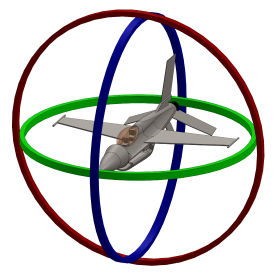
\includegraphics[width=\textwidth]{figs/gimbal}
\caption{3-Axis gimbal}
\label{fig:gimbal}
\end{subfigure}
\begin{subfigure}{0.5\textwidth}
\centering
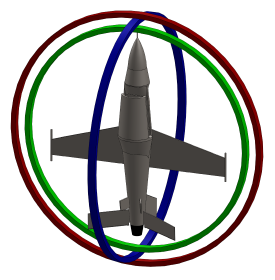
\includegraphics[width=\textwidth]{figs/gimbal-lock}
\caption{Locked gimbal with loss of DOF}
\label{fig:gimbal-lock}
\end{subfigure}
\caption{Mechanical gimbal lock}
\end{figure} 
\par
What is clear in the physical world is not necessarily as clear mathematically. An obvious loss of differentiability is present in the Euler Matrix $\Psi(\eta)$, defined previously in Eq:\ref{eq:angular-rates.e} from Sec:\ref{subsec:proto.conventions.frames}. That relation between angular velocity, in the inertial frame or inversely in the body frame, and the angular rates of the Euler Angles is dependent on singular secant and tangential terms.
\begin{equation}\label{eq:euler-derivative}
\begin{bmatrix}
\dot{\phi}\\
\dot{\theta}\\
\dot{\psi}
\end{bmatrix}
=\begin{bmatrix}
1 & sin(\phi)tan(\theta) & cos(\phi)tan(\theta)\\
0 & cos(\phi) & -sin(\phi)\\
0 & sin(\phi)sec(\theta) & cos(\phi)sec(\theta)\\
\end{bmatrix}
\begin{bmatrix}
p\\
q\\
r
\end{bmatrix}
=\Phi(\eta)\omega_b
\end{equation}
\begin{equation}
\text{As}~\underset{{\theta \rightarrow \pi /2}}{lim}~sec(\theta),tan(\theta)\rightarrow \infty
\end{equation}
Or that $\Phi(\eta)$ is undefined at $\theta=\pi/2$. 
It's clear to see that in Eq:\ref{eq:euler-derivative} there exists an undefined singularity as $\theta\rightarrow\pi/2$. The physical consequence of this is the loss of a degree of freedom. More specifically, if one looks at how the Z-Y-X rotation (or transformation) matrices are formulated:
\begin{subequations}
\begin{equation}
\mathbb{R}_I^b = \mathbb{R}_z\mathbb{R}_y\mathbb{R}_x=\begin{bmatrix}
c_\psi & -s_\psi & 0\\
s_\psi & c_\psi & 0\\
0 & 0 & 1
\end{bmatrix}
\begin{bmatrix}
c_\theta & 0 & s_\theta\\
0 & 1 & 0\\
-s_\theta & 0 & c_\theta
\end{bmatrix}
\begin{bmatrix}
1 & 0 & 0\\
0 & c_\phi & -s_\phi\\
0 & s_\phi & c_\phi
\end{bmatrix}
\end{equation}
\begin{equation}
\mathbb{R}_I^b=\begin{bmatrix}
c_\psi c_\theta & c_\psi s_\theta s_\phi - s_\psi c_\phi & c_\psi s_\theta c_\phi + s_\psi s_\phi\\
s_\psi c_\theta & s_\psi s_\theta s_\phi + c_\psi c_\phi & s_\psi s_\theta  c_\phi - c_\psi s_\phi\\
-s_\theta & c_\theta s_\phi & c_\phi c_\theta\\
\end{bmatrix}
\end{equation}
In the case where $\theta=\pi/2$, and using trigonometric double angles, the following can be reduced;
\begin{equation}\label{eq:gimbal}
=\begin{bmatrix}
0 & c_\psi s_\phi - s_\psi c_\phi & c_\psi c_\phi + s_\psi s_\phi\\
0 & s_\psi s_\phi + c_\psi c_\phi & s_\psi c_\phi - c_\psi s_\phi\\
-1 & 0 & 0\\
\end{bmatrix}
=
\begin{bmatrix}
0 & s(\phi - \psi) & c(\phi - \psi)\\
0 & c(\phi - \psi) & s(\phi - \psi)\\
-1 & 0 & 0
\end{bmatrix}=\mathbb{R}_{x'}(\phi-\psi)
\end{equation}
\end{subequations}
Where the resultant in Eq:\ref{eq:gimbal} represents an $\hat{X}'$-axis rotation in a new intermediate frame, post a $\pi/2$ rotation about the $\hat{Y}$-axis. Through trigonometric double angles a degree of freedom is lost at $\theta=\pi/2$, when $\phi$ \& $\psi$ effect the same angle.
%====================================================
\subsection{Quaternion Dynamics}
\label{subsec:dynamics.rigidbody.quaternion}
%====================================================
An algorithm proposed in \emph{How To Avoid a Singularity When Using Euler Angles?}\cite{euleranglesingularity} suggested a solution to the problem of Euler Angle singularities. The heuristic proposed was to switch between sequencing conventions (ZYX,ZYZ etc\ldots there are 12 in total) such that the singularity is always avoided. However the implementation of such an algorithm is cumbersome and inefficient. Far more elegant is the use of \emph{quaternion} attitude representations in $\mathbb{R}^4$ (\cite{rotationsequences,quaterniondynamics,spacecraftattitutdequaternions} amongst others\ldots most notably made popular by Shoemake [1987]\cite{shoemake} for use in animation).
\par
A quaternion is analogous to a rotation matrix in that it represents an attitude difference between two reference frames. An $\mathbb{R}^3$ position is paramterized as one rotation $\theta$ about a single unit \emph{Euler} axis $\hat{u}$ (sic Rodriguez Formula\cite{unwinding}). Without deliberating too much on their proof or details, a quaternion consists or a scalar component, $q_0$, and complex vector component, $\vec{q}\in \mathbb{C}^3$, such that;
\begin{equation}
Q\triangleq 
\begin{bmatrix}
q_0 \\
\vec{q}
\end{bmatrix}
~~\in\mathbb{R}^4
\end{equation}
The relationship between an Euler Angles rotation matrix $\mathbb{R}_I^b(\eta)$ and a quaternion attitude $Q_b$ is given by the Rodriguez formula:
\begin{equation}\label{eq:rodriguez}
\mathbb{R}_I^b(\eta)=\mathbb{R}(Q_b)=\mathbb{I}+2q_0[\vec{q}\hspace{2pt}]_\times+2[\vec{q}\hspace{2pt}]_\times\text{}^2
\end{equation}
Any and all quaternions, unless otherwise stated, in this dissertation are unit quaternions\footnote{Unit quaternions are a subset of the quaternion space}, $Q\in\mathbb{Q}_u$. The need for quaternions with unity magnitude is such to ensure rotational operations don't affect the magnitude of the vector operand. A unit quaternion is defined as:
\begin{equation}
\norm{Q}=\sqrt{{q_0}^2+\vec{q}\text{}\hspace{2pt}^2}=1
\end{equation}
Quaternion multiplication is distributive and associative, but not commutative. Specifically a quaternion multiplciation operation is equivalent to the Hamilton product. For two quaternions, $Q$ \& $P$:
\begin{subequations}
\begin{equation}
Q\otimes P = \begin{bmatrix}
q_0 \\
\vec{q}
\end{bmatrix}
\otimes
\begin{bmatrix}
p_0 \\
\vec{p}
\end{bmatrix}
\end{equation}
\vspace{-5pt}
\begin{equation}\label{eq:quaternion-product}
=q_0 p_0 - \vec{q}\cdot \vec{p}+p_0 \vec{q} + q_0 \vec{p} + \vec{q}\times\vec{p}
\end{equation}
\end{subequations}
Seeing that the vector component of a quaternion is complex valued, it is natural that there exists a quaternion conjugate property. Namely:
\begin{equation}
Q^*=\begin{bmatrix}
q_0 \\
-\vec{q}
\end{bmatrix}
\end{equation}
It then follows that\footnote{Disambiguation: $\mathbb{I}$ in this context is a $4\times 4$ identity matrix, not an inertial matrix} the fundamental quaternion identity is:
\begin{equation}
Q\otimes Q^* = \mathbb{I}_{4\times 4}
\end{equation}
Application of a right handed quaternion rotation to a vector $\vec{v} \in\mathbb{R}^3$ involves multiplication by two unit quaternions. 
\begin{equation}
\begin{bmatrix}
0 \\
\vec{v}\hspace{2pt}'
\end{bmatrix}
=Q\otimes
\begin{bmatrix}
0 \\
\vec{v}
\end{bmatrix}
\otimes Q^*
\end{equation}
Mostly, the zero scalar components are omitted in a rotation (\emph{or transformation}) operation, as such it is implied vector operands are substituted with quaternions.
\begin{equation}\label{eq:quaternion-rotation}
\vec{v}\hspace{2pt}'=Q \otimes (\vec{v}\hspace{2pt}) \otimes Q^*
\end{equation} 
In the case of rigid body attitude representation, $Q_b$ is the quaternion which represents the difference between $\mathcal{F}^b$ and $\mathcal{F}^I$. A quaternion operator is equivalent to a rotation matrix operation:
\begin{equation}
\mathbb{R}_I^b \underset{Q}{\iff} Q_b \otimes (.) \otimes Q_b^*
\end{equation}
A Z-Y-X sequenced\footnote{The resultant quaternion rotational products are sequence independent, but the quaternions rotational trajectories do depend on the sequence used. Here they are sequenced following the order of the rotational Euler angles used as arguments.} body quaternion, $Q_b$, can be constructed from Euler angles as:
\begin{equation}\label{eq:quaternion-sequence}
Q_b=Q_z\circ Q_y\circ Qx=\begin{bmatrix}
cos(\psi/2)\\
0\\
0\\
sin(\psi/2)
\end{bmatrix}
\otimes
\begin{bmatrix}
cos(\theta/2)\\
0\\
sin(\theta/2)\\
0
\end{bmatrix}
\otimes
\begin{bmatrix}
cos(\phi/2)\\
sin(\phi/2)\\
0\\
0
\end{bmatrix}
\end{equation}
A quaternion time derivative, with $Q_\omega$ being a quaternion with a vector component equal to angular velocity $\vec{\omega}_{b/I}$ and a zero scalar component, is given by:
\begin{equation}\label{eq:quaternion-deriv}
\frac{d}{dt}Q_b=\frac{1}{2}Q_b\otimes Q_{\omega}=\begin{bmatrix}
-\frac{1}{2}\vec{q}\hspace{2pt}^{T} \vec{\omega}_b\\
\frac{1}{2}\big([\vec{q}\hspace{2pt}]_\times+q_0\mathbb{I}\big)\vec{\omega}_b
\end{bmatrix}
\end{equation}
Using quaternions to represent attitudes negates the need for an Euler Matrix, $\Phi(\eta)$, to represent attitudes and their rates. A body quaternion is fully defined in the inertial frame with respect to the body frame or inversely so. The first quaternion time derivative replaces Eq:\ref{eq:states.a} \& Eq:\ref{eq:states.c};
\begin{subequations}
\begin{equation}
\dot{\mathcal{E}}=\mathbb{R}_b^I(-\eta)\vec{\nu}\underset{Q}{\iff}Q_b(-\eta)\otimes\vec{\nu}\otimes Q_b(-\eta)^*=Q_b^*\otimes \vec{\eta} \otimes Q_b~~~~\in\mathcal{F}^I
\end{equation}
\vspace{-10pt}
\begin{equation}
\dot{\eta}=\Phi(\eta)\vec{\omega}_b\underset{Q}{\iff}\dot{Q}=\frac{1}{2}Q_b\otimes Q_\omega~~~~\in\mathcal{F}^{v2,v1,I}
\end{equation}
\end{subequations}
Second order time derivatives for quaternion acceleration aren't as useful or concise as their higher order velocity counterparts. The second order derivative is provided here however it's only relevant to quaternion backstepping later in the control chapter. If possible, quaternion accelerations are mostly avoided due to the complexity of their evaluation;
\begin{equation}
\ddot{Q}\big(\dot{Q},Q,t)=\dot{Q}\otimes Q^* \otimes \dot{Q}+\frac{1}{2}Q\otimes \big[\mathbb{I}_b^{-1}(\tau-4(Q^*\otimes \dot{Q})\times(\mathbb{I}_b(Q^*\otimes \dot{Q}))\big]
\end{equation}
%====================================================
\subsection{Quaternion Unwinding}
\label{subsec:dynamics.rigidbody.unwinding}
%====================================================
Although quaternions are indeed better than Euler angles, lacking the associated singularity, they do contain one caveat. Seeing that a quaternion $Q=[q_0~\vec{q}\hspace{2pt}]^T$ represents an attitude orientation of a body in $\mathbb{R}^3$ using $\mathbb{R}^4$ variables there exists what is called a dual coverage\cite{unwinding}. Each unit quaternion, stemming from Euler-Rodriguez theorem, is parametrized such that the quaternion operation represents a single Euler-axis rotation of $\theta$ about a unit axis $\hat{u}$ such that:
\begin{equation}
Q=\begin{bmatrix}
q_0\\
\vec{q}
\end{bmatrix}=
\begin{bmatrix}
cos(\theta/2)\\
sin(\theta/2)\hat{u}
\end{bmatrix}
\end{equation}
That rotation is applied with a quaternion operator Eq:\ref{eq:quaternion-rotation}. In then follows that for each unique attitude in 3-Dimensions there exist two quaternions which correlate to the same position, differing by their rotational direction about the Euler-axis. Seeing that $\theta=2\pi-\theta$\footnote{Disambiguation: $\theta$ is not the $\hat{Y}$-axis Euler angle here\ldots}, then there are two definitions for $Q_b$;
\begin{subequations}
\begin{equation}
Q_b =
\begin{bmatrix}
q_0 \\
\vec{q}
\end{bmatrix}
=
\begin{bmatrix}
cos(\theta/2)\\
sin(\theta/2)\hat{u}
\end{bmatrix}
\end{equation}
\vspace{-6pt}
\begin{equation}
Q=\begin{bmatrix}
cos(\pi - \theta/2)\\
sin(\pi - \theta/2)\hat{u}
\end{bmatrix}
=
\begin{bmatrix}
-cos(\theta/2)\\
sin(\theta/2)\hat{u}
\end{bmatrix}
\end{equation}
\vspace{-6pt}
\begin{equation}\label{eq:euler-quaternion}
\eta\in\mathbb{R}^3\underset{Q}{\iff}\begin{bmatrix}
\pm q_0\\
\vec{q}
\end{bmatrix}
\in\mathbb{R}^4
\end{equation}
\end{subequations}
The conjecture in Eq:\ref{eq:euler-quaternion} is that for each physical attitude in $\mathbb{R}^3$ there are two corresponding quaternions in $\mathbb{R}^4$; $[\pm q_0~\vec{q}~]^T$. A consequence of this is two possible error state trajectories for every attitude difference. Both a clockwise $\theta$ rotation and an anticlockwise $2\pi-\theta$ negative rotation will point to the same quaternion error state. This could lead to an erroneous and unnecessary "unwinding" of a complete counter revolution as a result of a dual covered error state. 
\par
Often the signed scalar component of the attitude quaternion error (Sec:\ref{subsec:control.attitude.problem}) is simply neglected or assumed positive. As such for attitude controllers the requirement is that for positive and negative scalars the control input is consistent:
\begin{equation}
\nu_d=h([q_0~\vec{q}\hspace{2pt}]^T,t)=h([-q_0~\vec{q}\hspace{2pt}]^T,t)
\end{equation}
Or more simply that $Q_e=[|q_0|~\vec{q}\hspace{2pt}]^T$. The most simple solution adhering to that constraint, which control designers often adopt, is to simply neglect the scalar component altogether. The adjustment is to use a simplified error state argument for the control law; $h(\vec{q}_e,t)$. Such a solution is an oversimplification and would only ever be asymptotically stable in the local and not global regions. 
\par
An alternative solution is using an only positive quaternion scalar, one that will always ensure that an error state represents a right-handed clockwise rotation and not necessarily the most direct rotation trajectory. If the resolution of trajectory co-ordinates generated is sufficiently high enough, the control plant will however never encounter a problem. One proposal in \emph{Nonlinear Quadcopter Attitude Control}\cite{nonlinearquadcopter} suggested using a \emph{signum} operator to design the signs of the controller coefficients for the virtual control plant input. 
\begin{subequations}\label{eq:signum-unwinding}
\begin{equation}
\vec{\omega}_d=\frac{2}{\tau}sgn(q_0)\vec{q}
\end{equation}
\begin{equation}
sgn(\vec{q})=
\begin{cases}\begin{array}{ll}
1 & ~~\vec{q}\geq 0\\
-1 & ~~\vec{q}< 0\\
\end{array}
\end{cases}
\end{equation}
\end{subequations}
The resultant \emph{hybrid} mode controller provides global asymptotic stability, but only in the case that the Euler-axis angle $\theta\leq \pm\pi$. The control law described in Eq:\ref{eq:signum-unwinding} would still need the control torques to be designed from that angular velocity virtual control setpoint.
\par
Another proposal \cite{unwinding} to the unwinding problem was to lift the quaternion error-state back into $\mathbb{R}^3$ using the Rodriguez formula, Eq:\ref{eq:rodriguez}. The mapping back to $\mathbb{R}^3$ effectively ensures that $\theta$ is minimized, or that the error-state imposes the shortest possible rotation between the reference and desired body frames. Controllers presented in Sec:\ref{sec:control.attitude} all incorporate the signed quaternion scalar into the control law;  hence relying on the trajectory generation to provide the desired direction of the rotation path.
%====================================================
\section{Multibody Nonlinearities}
\label{sec:dynamics.nonlinearities}
%====================================================
Typically multibody dynamics are solved (and simulated) as a series of torque \& force interactions or responses. There are many different schools of thought on the subject which each have proposed various methodologies for stepping through the systems dynamics [sic Implicit Euler\cite{physicallybased,multibodydynamics} or otherwise \ldots]. For the prototype design here, only relative rotational motion is permissible between the interconnected rigid bodies. Each body is considered independently, as free and rigid, whose constraint torques induced from excitation are imposed onto sequential rotational joints. Opposed to those torques are Newtonian responses of importance which manifest as what are termed \emph{gyroscopic} and \emph{inertial} torques. Those responses are now quantified and introduced into the dynamic model derived in Sec:\ref{subsec:dynamics.rigidbody.lagrange}. By the nature of the design there can be no unbalanced constraining forces existing between each body and as such the translational model is regarded as rigid.
\par
A distinction must be made between torque responses here and those of Eq:\ref{eq:states.d}. The latter being a response to be diminished in feedback compensation and the former being something which is later exploited by the control allocation algorithm in a feedforward type configuration, Sec:\ref{sec:control.allocation}. The multibody analysis which follows is a very Newtonian approach in that each body involved is resolved independently and relative responses are transformed onto the inducing body. The alternative numeric solution is to form a Lagrangian for the entire dynamic system, this would simplify solving net effects. Such an approach is unused here as each individual effect needs to be quantified if they're to be used as potential actuator inputs.
%====================================================
\subsection{Relative Rotational Gyroscopic \& Inertial Torques}
\label{subsec:dynamics.nonlinearities.gyrotorques}
%====================================================
The torque responses induced from relative rotations, the only permissible intra-body movement, are transferred from the interacting bodies as a result of Newtons second law of rotational motion. For each of the motor modules' pitching or rolling motion, the respective servo motors apply some torque to invoke that rotation. Opposed to the rotational motion are both inertial and gyroscopic response(s) of that body being acted upon. The latter being a consequence of a vector's time derivative in a rotating frame, Eq:\ref{eq:reynolds}.
\par
Each of the four motor modules are symmetrical and as such the induced torque response characteristics for one module can be extrapolated through a reference frame rotation. Seeing that each relative rotation from the actuator set $u\in\mathbb{U}$ is actuated independently and upon a different body, their responses are calculated separately too.
\par
Drawing again from Lagrangian theory\footnote{The generalized linear kinetic energy for each module is an extension of that in Eq:\ref{eq:rigid-frame.a} and is independent of any of the actuator positions.} and considering only the rotational kinetic energy for the inner ring assembly $\mathcal{F}^{M_i}$. There are no permissible transnational motions between each body and as such there can be no linear kinetic energy contribution. The Lagrangian for the inner ring is formed, with concern on the effect $\lambda_i$ has on the system:
\begin{equation}
\mathcal{L}_{M_i}=\frac{1}{2}\vec{\Omega}_i\text{}^T\big(\mathbb{I}_{p}\big)\vec{\Omega}_i+\frac{1}{2}\dot{\vec{\lambda}}_i\text{}^T\big(\mathbb{I}_{\lambda}\big)\dot{\vec{\lambda}}_i
\end{equation}
Where $\mathbb{I}_p$ is the propeller's rotational inertia, Eq:\ref{eq:inertia-prop}, and $\mathbb{I}_\lambda$ being the inner ring's inertia, defined in Eq:\ref{eq:inertia.inner.a}. Noting that $\vec{\Omega}_i=[0~~0~~\Omega_i]^T\in\mathcal{F}^{M_i}$ and $\dot{\vec{\lambda}}_i=[\dot{\lambda}_i~~0~~0]^T\in\mathcal{F}^{M_i'}$, the two contributors are not in a common frame. As such the equation \footnote{The transformation of $\dot{\vec{\lambda}}_i\rightarrow\dot{\vec{\lambda}}_i'$ is superfluous but included for completeness.} changes to:
\begin{subequations}
\begin{equation}
\mathcal{L}_{M_i}=\frac{1}{2}\vec{\Omega}_i\text{}^T\big(\mathbb{I}_{p}\big)\vec{\Omega}_i+\frac{1}{2}\dot{\vec{\lambda}}_i'\text{}^T\big(\mathbb{I}_{\lambda}\big)\dot{\vec{\lambda}}_i'
\end{equation}
\vspace{-10pt}
\begin{equation}
\dot{\vec{\lambda}}_i'=Q_x(-\lambda_i)\otimes\big(\dot{\vec{\lambda}}_i\big)\otimes Q_x^*(-\lambda_i)\Rightarrow \dot{\vec{\lambda}}_i'=\dot{\vec{\lambda}}_i
\end{equation}
\end{subequations}
Where both $\mathbb{I}_{p}$ and $\mathbb{I}_{\lambda}$ are taken W.R.T to their rotational centre(s).
\par
Then recalling the Euler-Lagrange formulation from Eq:\ref{eq:euler-lagrange} with generalized co-ordinates\footnote{Relative to the body frame and not the inertial frame because Eq:\ref{eq:states.d} accounts for the inertial response of the entire body frame. Here only the induced relative responses are being considered.} $\mathbf{u}(t)$ for the motor module frame, $\mathcal{F}^{M_i}$, relative to  the body frame, $\mathcal{F}^b$.
\begin{equation}
\frac{d}{dt}\bigg(\frac{\delta L}{\delta \dot{\mathbf{u}}}\bigg)-\frac{\delta L}{\delta \mathbf{u}} = \mathbf{V} = \vec{\tau}_{net}
\end{equation}
It then follows that:
\begin{subequations}
\begin{equation}
\frac{d}{dt_b}\bigg(\frac{\delta\mathcal{L}}{\delta\dot{\mathbf{u}}}\bigg)=\frac{d}{dt_{M_i}}\mathbb{I}_p\vec{\Omega}_i+\vec{\omega}_{M_i/b}\times\mathbb{I}_p\vec{\Omega}_i+\frac{d}{dt_{M_i}}\mathbb{I}_{\lambda}\dot{\vec{\lambda}}_i+\vec{\omega}_{M_i/b}\times\mathbb{I}_{\lambda}\dot{\vec{\lambda}}_i
\end{equation}
With $\vec{\omega}_{M_i/b}$ being the net angular velocity of the inner ring frame relative to the body frame. Both inner and middle ring servo rates, $d\vec{\lambda}_i/dt$ \& $d\vec{\alpha}_i/dt$ respectively, contribute to that inner ring's relative angular velocity:
\begin{equation}
\vec{\omega}_{M_i/b}= Q_x(-\lambda_i)Q_y(-\alpha_i)\otimes\dot{\vec{\alpha}}_i\otimes Q_y^*(-\alpha_i)Q_x^*(-\lambda_i)+Q_x(-\lambda_i)\otimes\dot{\vec{\lambda}}_i\otimes Q_x^*(-\lambda_i)
\end{equation}
The net torque from a $\lambda_i$ rotation, induced in the motor module frame $\mathcal{F}^{M_i}$, can be grouped into second order \emph{Inertial} and first order \emph{Gyroscopic} components. Depending on the fidelity of the model or aggressiveness of control actions taken, higher order induced terms could be ignored to save computational complexity.
\begin{equation}\label{eq:torque-induced-inner}
\vec{\tau}_\lambda=\underbrace{\mathbb{I}_p\dot{\vec{\Omega}}_i+\mathbb{I}_{\lambda}\ddot{\vec{\lambda}}_i}_{Inertial}+\underbrace{\vec{\omega}_{M_i/b}\times\mathbb{I}_p\vec{\Omega}_i+\vec{\omega}_{M_i/b}\times\mathbb{I}_{\lambda}\dot{\vec{\lambda}}_i}_{Gyroscopic}~~~~\in\mathcal{F}^{M_i}
\end{equation}
\end{subequations}
Similarly for the middle ring, with the inertia, $\mathbb{I}_{\alpha}(\lambda_i)$, as a function of the inner ring rotation angle, $\lambda$, from Eq:\ref{eq:inertia.middle.c}. Using a new set of generalized co-ordinates, $\mathbf{v}(t)$, for the middle ring frame, $\mathcal{F}^{M_i'}$, relative to the body frame, the Lagrangian is then:
\begin{subequations}
\vspace{-8pt}
\begin{equation}
\mathcal{L}_{M_i'}=\frac{1}{2}\dot{\vec{\alpha}}_i\text{}^T\big(\mathbb{I}_{\alpha}(\lambda_i)\big)\dot{\vec{\alpha}}_i
\end{equation}
\vspace{-10pt}
\begin{equation}
\frac{d}{dt_b}\bigg(\frac{\delta L}{\delta \dot{\mathbf{v}}}\bigg) = \frac{d}{dt_{M_i'}}\mathbb{I}_\alpha(\lambda_i)\dot{\vec{\alpha}}_i+\vec{\omega}_{M_i'/b}\times\mathbb{I}_\alpha(\lambda_i)\dot{\vec{\alpha}}_i
\end{equation}
\vspace{-6pt}
\begin{equation}
\vec{\omega}_{M_i'/b}=Q_y(-\alpha_i)\otimes\dot{\vec{\alpha}}_i\otimes Q_y^*(\alpha_i)
\end{equation}
Which are similarly grouped into first and second order gyroscopic and inertial components.
\begin{equation} \label{eq:torque-induced-middle}
\vec{\tau}_\alpha(\lambda_i)=\underbrace{\mathbb{I}_{\alpha}(\lambda_i)\ddot{\vec{\alpha}}_i}_{Inertial}+\underbrace{\vec{\omega}_{M_i'/I}\times\mathbb{I}_{\alpha}(\lambda_i)\dot{\vec{\alpha}}_i}_{Gyroscopic}~~~~\in\mathcal{F}^{M_i'}
\end{equation}
\end{subequations}
\par
\begin{figure}[hbtp]
\vspace{-20pt}
\centering
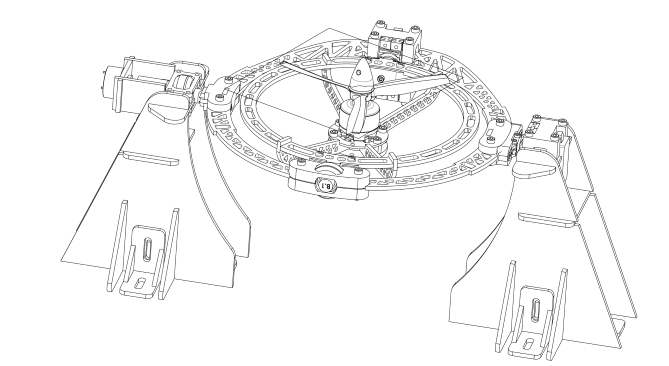
\includegraphics[width=0.6\textwidth]{figs/torque-response}
\caption{Torque response rig}
\label{fig:torque-response}
\end{figure}
Each of the induced torques, $\vec{\tau}_\lambda$ and $\vec{\tau}_\alpha(\lambda_i)$, occur in intermediary frames associated with the inner and middle ring assemblies. As such, their negative responses effect\footnote{Depending on dynamic equations used it could  effect Eq:\ref{eq:rigid-frame.b}. However the equations Eq:\ref{eq:rigid-frame} are unnecessary when using quaternion dynamics.} Eq:\ref{eq:states.d}, and each need to be transformed to the body frame.
\begin{equation}\label{eq:torque-response}
\vec{\tau}_Q(u)=\sum_{i=1}^4 -Q_{M_i}^*\otimes \vec{\tau}_{\lambda_i}(u)\otimes Q_{M_i}-Q_{M_i'}^*\otimes \vec{\tau}_{\alpha_i}(u) \otimes Q_{M_i'}~~~\in\mathcal{F}^b
\end{equation}
\par
The torque response equations where tested using the rig in Fig:\ref{fig:torque-response}. The first plot in Fig:\ref{fig:tau-lambda} shows the induced torque for $\tau_\lambda$ measured purely about the $\hat{X}_{M_i}$ axis. The plot changes with increased rotation rates of $\Omega_i$\footnote{Motors 1 \& 3 have clockwise rotations ('+'), motors 2 \& 4 are counter-clockwise ('-').}, illustrating the gyroscopic torque effect from the propeller's rotation. Plotted against measured values are $\hat{\tau}_\lambda$ estimates from Eq:\ref{eq:torque-induced-inner}. Similarly the second plot in Fig:\ref{fig:tau-alpha} shows the middle ring induced torque, $\tau_\alpha\in\mathcal{F}^{M_i'}$. Detailing variations with respect to changing $\lambda_i$ positions. The changes in $\mathbb{I}_\alpha(\lambda_i)$ alter the magnitude of torque responses inline with estimates of $\hat{\tau}_\alpha$.
\begin{figure}[hbtp]
\begin{subfigure}{0.5\textwidth}
\centering
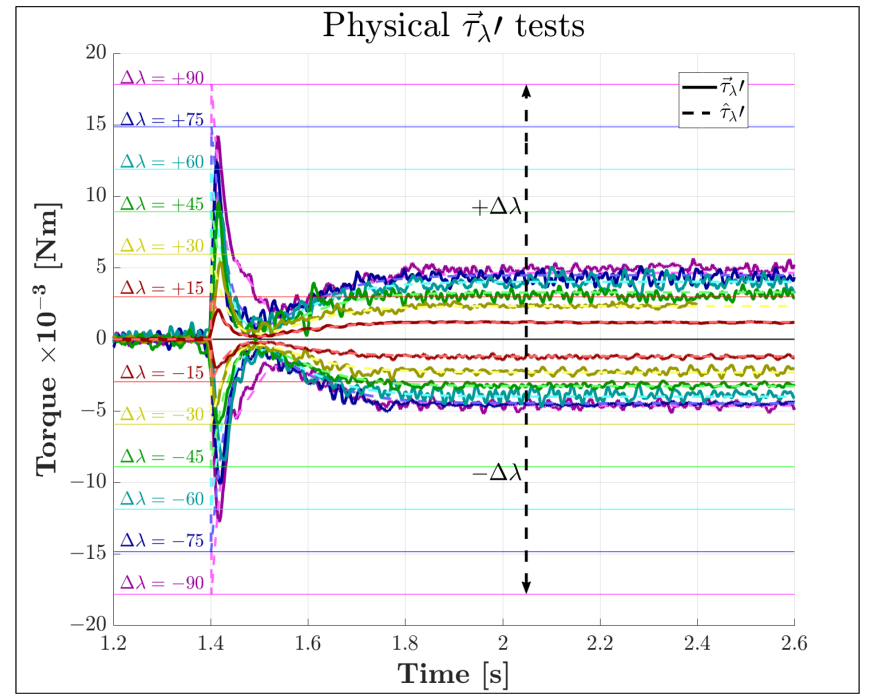
\includegraphics[width=\textwidth]{graphs/tau-lambda}
\caption{$\tau_\lambda$ variations with propeller speeds $\Omega_i$}
\label{fig:tau-lambda}
\end{subfigure}
\begin{subfigure}{0.5\textwidth}
\centering
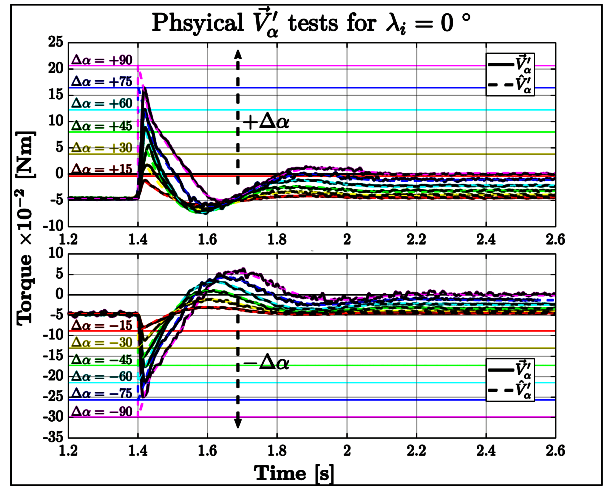
\includegraphics[width=\textwidth]{graphs/tau-alpha}
\caption{$\tau_\alpha$ variations with changing $\mathbb{I}_\alpha(\lambda_i)$}
\label{fig:tau-alpha}
\end{subfigure}
\vspace{-5pt}
\caption{Torque responses for inner and middle rings}
\vspace{-10pt}
\end{figure}
\par
\emph{\color{Gray}The above responses are pertinent to simulation and plant dependent feedback compensation. The simulation environment is structured such that the torques are produced as responses from Newtonian movement at every step interval. In due course it would be more efficient (and less stiff) for the simulation to exploit an implicit Euler\cite{physicallybased,multibodydynamics} coordinate system in lieu of the cartesian response equations developed above. However this was not implemented in Chapter:\ref{ch:simulation} and remains open to further testing and simulation\ldots}
%====================================================
\section{Aerodynamics}
\label{sec:dynamics.aero}
%====================================================
The relationship between a propeller's rotational speed, $\Omega_i$, and its produced thrust, $\vec{T}(\Omega_i)$, is more complicated than the quadratic simplification taken at static conditions which most papers puport. Thrust induced is mostly dependent on the incident air stream flowing into the propellers rotational plane; typically being the component of the body velocity normal to that propeller's plane (Eq:\ref{eq:normal-fluid}). Parallel fluid flowing across the propeller contributes toward in-plane aerodynamic drag (hence torque). 
\par
The combination of aerodynamic Blade-element\cite{bem,forwarddescent} and fluid-dynamics Momentum (\emph{disc actuator}) theories stipulates an integral term taken across the propellers length which accurately models the produced thrust and torque. A verbose presentation of all aerodynamic effects experienced by a quadrotor's propeller(s) is thoroughly detailed in \cite{bladesforquadrotors} and again \cite{nonlineardynamics}. The following provides a review of pertinent aerodynamic theories. Some phenomena aren't included, like Vortex Ring States or parasitic drag like effects, which weren't deemed to be pertinent.
%====================================================
\subsection{Propeller Torque and Thrust}
\label{subsec:dynamics.aero.bem}
%====================================================
\emph{\color{Gray} A feasible situation which the prototype could encounter is where an upstream propeller provides the incident fluid flow to another downstream propeller. Such a situation presents a complicated fluid dynamics \& vortex wake effect problem. Propeller overlapping effects are investigated in \cite{configurationpropulsion}, but remain open to further research in the context of the aircraft considered here.}
\par
\emph{\color{Gray}To expedite the system ID process some simplifications are made on the aerodynamics to construct an approximate model; specifically using coefficients in place of complete local chord and pitch based integrals. Such an assumption holds true given that fixed pitch propellers are used.}
\par
\begin{figure}[htbp]
\centering
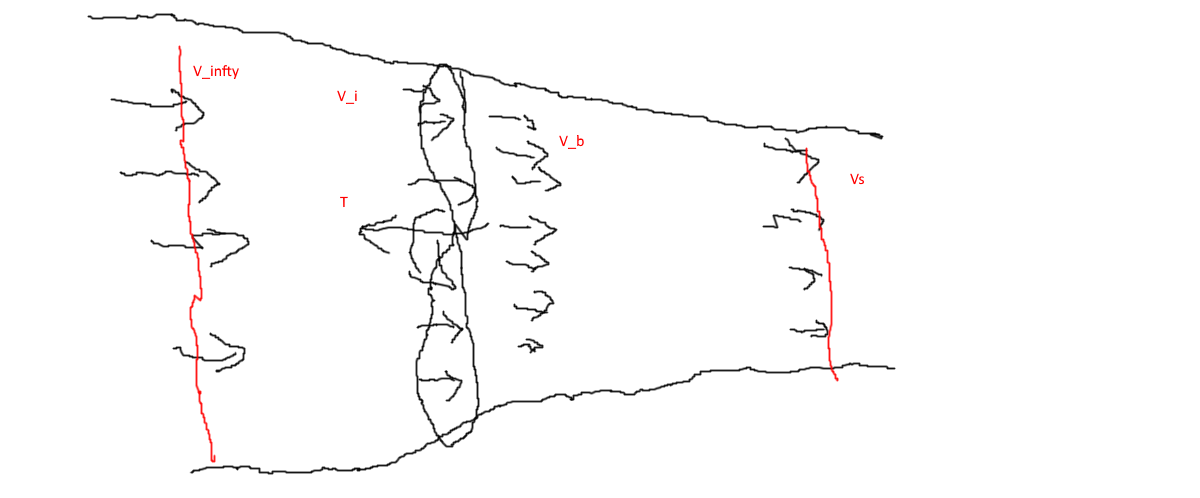
\includegraphics[width=0.75\textwidth]{figs/bem-flow}
\caption{Disc Actuator Propeller Planar Flow}
\label{fig:bem-flow}
\end{figure}
The rotation of a propeller applies a thrust force, $\vec{T}$, onto the fluid stream\footnote{Only perpendicular mass flow across the propeller's plane is considered for momentum theory, adjacent fluid velocities are small enough that propeller induced drag is neglected\ldots} in which it acts. That fluid stream (Fig:\ref{fig:bem-flow}) has an incident head velocity, $v_\infty$, and a resultant slip velocity downstream relative to the rotational plane, $v_s$. There exists some relationship about the change of fluid flow applied by the propeller's rotation. Such a relationship can then be given by:
\begin{equation}
v_ s = \Delta v + v_\infty
\end{equation}
Wherein $\Delta v$ is the change in velocity, added to the fluid by the propeller blade's rotating aerofoil profile. The propeller induces a velocity directly in front of it's rotational plane, $v_i$, such that the net fluid flow into the plane is $v_b=v_i+v_\infty$. Bernoulli's principle$^{\dagger}$ has it that net fluid flow through that plane is:
\begin{equation}\label{eq:bernoulli}
v_b = \frac{1}{2} ( v_s - v_{\infty} ) = \frac{1}{2} \Delta v = \frac{1}{2} v_s \big|_{v_\infty=0}
\end{equation}
\par
And as such, stemming from classical Disc Actuator$^{\dagger}$ (fluid \emph{momentum}) theory, the \underline{scalar} force, $T(\Omega)$, acting on the fluid is calculated as a function of mass flow rate with respect to the change in fluid velocity (pressure differential).
\begin{equation}\label{eq:prop-mass}
T=(A_b v_b)\Delta v = \rho \pi R_b^2v_b \Delta v = \rho \pi R_b^2(v_i+v_\infty)\Delta v = \frac{1}{2} \rho \pi R_b^2 \Delta v^2
\end{equation}
Where $R_b$ is the disc (propeller) radius for the fluid stream under consideration. The fluid density of that stream, $\rho$, is typically $1.225 Kg.m^{-3}$. The solution to Eq:\ref{eq:prop-mass} is not entirely clear in terms of $\Omega_i$, which is the desired form in which the thrust can be calculated. It can however be solved as a function of aerodynamic propulsive power expended, $\Delta P=\vec{T}\Delta v$. That kinetic energy relationship between rotational kinetic energy and power transferred from the motor is tenuous at best, compounded by parasitic losses which deteriorate the power transferred through the propellers. Furthermore, the local fluid velocity through the propeller isn't purely normal to its plane. 
\par
The fluid flow induced by the propeller's rotation directly in front of its plane of rotation is not purely perpendicular but has axial and tangential induced velocity components, $a$ and $a'$ respectively. Those induced components for the fluid velocity can be abstracted to induction factors dependent on the incident fluid velocity to the propeller's plane of rotation:
\begin{subequations}\label{eq:induction-factors}
\vspace{-5pt}
\begin{equation}\label{eq:induction-axial}
v_i=a v_\infty~~\text{in the axial direction}
\end{equation}
\vspace{-20pt}
\begin{equation}\label{eq:induction-tangential}
v_\theta=a' \Omega_i R_b~~\text{in the tangential direction}
\end{equation}
\end{subequations}
From induction factors defined Eq:\ref{eq:induction-factors}, the velocity components can be written as functions of free upstream velocity $v_\infty$.
\begin{subequations}
\vspace{-5pt}
\begin{equation}
v_b=(1+a)v_\infty
\end{equation}
\vspace{-15pt}
\begin{equation}
v_s=(1+2a)v_\infty
\end{equation}
\end{subequations}
A consequence of the tangential fluid flow is that there exists an angular momentum flow rate across the propeller plane. This results in a torque response to the rotational motion about the propeller's axis of rotation, analogous to Eq:\ref{eq:prop-mass}.
\\
\vspace{-10pt}
\begin{equation}\label{eq:prop-moment}
\vec{Q}=\rho\pi R_b^3 (v_\theta-v_\infty) v_b 
\end{equation}
\begin{figure}[hbtp]
\vspace{-15pt}
\centering
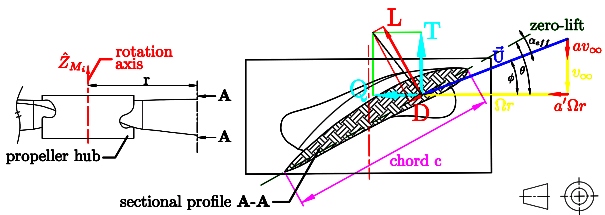
\includegraphics[width=0.9\textwidth]{figs/bem-profile}
\caption{Blade element profile at radius r}
\label{fig:bem-profile}
\end{figure}
\par
Together, Eq:\ref{eq:prop-mass} \& Eq:\ref{eq:prop-moment} make up propeller momentum theory but cannot be solved on their own. Blade-element theory analyses incremental aerofoil sections of width $dr$ of the propeller profile (Fig:\ref{fig:bem-profile}) at some radius $r$. Net local fluid velocity across a single elemental aerofoil profile $\vec{U}$ is calculated as:
\begin{equation}
\vec{U}=\sqrt{(v_\infty+v_i)^2+(v_\Omega+v_\theta)^2}
\end{equation}
Each elemental profile, of chord length $c$, has a local pitch, $\theta$, of its aerofoil zero-lift line relative to the horizontal. Local fluid velocities (again in Fig:\ref{fig:bem-profile}) encountered by the propeller make their own an angle of attack $\phi$ such that:
\begin{equation}
\phi=\theta-\alpha_{effective}
\end{equation}
That local angle of attack changes with the inflow magnitude $v_\infty$ and the induced axial velocity $v_i$. That trigonometric ratio is given as:
\begin{equation}
\phi=tan^{-1}\bigg(\frac{v_\infty+v_i}{v_\Omega+v_\theta}\bigg)=tan^{-1}\bigg(\frac{v_\infty(1+a)}{\Omega r(1+a')}\bigg)
\end{equation}
The in-plane fluid flow $\vec{U}(r,\phi)$, for an element at radius $r$ with a local angle of attack $\phi$, then contributes towards elemental lift and drag forces as a function of aerofoil's dimensionless lift, $C_L$, and drag, $C_D$, coefficients\footnote{The lift and drag coefficients are determined by the aerofoil's characteristics, but would be constant across the length of a variable pitch, non-twisted hinged propeller\ldots}.
\begin{subequations}
\begin{equation}
\Delta L=\frac{1}{2}\rho \vec{U}(r,\phi)^2 c C_L
\end{equation}
\vspace{-10pt}
\begin{equation}
\Delta D=\frac{1}{2}\rho \vec{U}(r,\phi)^2 c C_D
\end{equation}
\end{subequations}
With air density $\rho$\footnote{Typically $\rho = 1.225 kg/m^3$} and local chord length $c$. Those lift and drag forces are taken as components parallel and perpendicular to the plane of rotation. Those components are then thrust $T$ and torque $F_x$ forces (Fig:\ref{fig:bem-profile}). The in-plane force $F_x$ applies an aerodynamic torque $Q$ as the force acts at a radius $r$.
\begin{subequations}
\begin{equation}\label{eq:element-thrust}
dT=\frac{1}{2}\rho\vec{U}(r,\phi)^2c\big(C_L cos(\phi)+C_D sin(\phi)\big).dr
\end{equation}
\vspace{-5pt}
\begin{equation}\label{eq:element-drag}
dF_x=\frac{1}{2}\rho\vec{U}(r,\phi)^2c\big(C_L sin(\phi)+C_D cos(\phi)\big).dr
\end{equation}
\vspace{-5pt}
\begin{equation}\label{eq:element-torque}
\rightarrow dQ = \frac{1}{2}\rho\vec{U}(r,\phi)^2c\big(C_L sin(\phi)+C_D cos(\phi)\big)r.dr
\end{equation}
\vspace{-10pt}
\begin{equation}\label{eq:element-power}
\rightarrow dP = \Omega r dF_x .dr
\end{equation}
\end{subequations}
\par
Typically a power term, Eq:\ref{eq:element-power}, is given in lieu of torque or drag terms, Eq:\ref{eq:element-torque} or Eq:\ref{eq:element-drag}. Then calculating forces and power terms as per momentum theory for each element, in terms of axial and tangential induction factors:
\begin{subequations}\label{eq:moment-thrust-element}
\begin{equation}
dT=\rho 4 \pi r^2 v_\infty(1+a)a.dr
\end{equation}
\vspace{-10pt}
\begin{equation}
dP=\rho 4 \pi r^2 v_\infty(1+a)\Omega r (1+a').dr
\end{equation}
\end{subequations}
\par
Finally equating momentum and element terms together produces the blade-element momentum equation(s) for thrust and power produced by a propeller. Following a few assumptions, most importantly that the lift coefficient $C_L$ is a linear function of the effective angle of attack $\alpha_{eff}$. The lift curve gradient , $a_L$, for an ideally twisted blade, like the fixed pitch propellers under consideration here, is typically $2\pi$ such that $C_L=2\pi(\theta-\phi)$. And assuming that tangentially induced velocities $v_\theta$ are small (or that the tangential induction factor $a'<<1$) when compared to the propeller's speed $\Omega r$. Similarly the net inflow and axial induced velocities $v_\infty + v_i<<\Omega r$.\footnote{Small angle approximations then apply to $cos(\phi+\alpha_{eff})\approx 1$ and $sin(\phi+\alpha_{eff})\approx \phi+\alpha_{eff}$}
\newpage
\begin{subequations}
\begin{equation}\label{eq:bem-thrust}
T=\int_{r=0}^R \frac{1}{2} a_L b c \rho (\Omega r)^2 \big(\theta-\frac{v_\infty+v_i}{\Omega r}\big).dr
\end{equation}
\vspace{-3pt}
\begin{equation}\label{eq:bem-power}
P=\int_{r=0}^R \frac{1}{2}a_L b c \rho (\Omega r)^3\bigg[\big(\theta-\frac{v_\infty+v_i}{\Omega r}\big)\big(\frac{v_\infty+v_i}{\Omega r}\big) + C_d\bigg].dr
\end{equation}
\end{subequations}
With $b$ being the number of propeller blades. Generally knowing exact pitch and chord values as a function $r/R$ is difficult and calculating integrals at each process step is cumbersome. Both Eq:\ref{eq:bem-thrust} \& Eq:\ref{eq:bem-power} can be solved by equating element and momentum terms (a full expansion is given in Appendix:\ref{app:equations.bem}). Often dimensionless thrust, torque and power coefficients are defined across the entire blade's length:
\begin{subequations}\label{eq:coefficients}
\begin{equation}\label{eq:thrust-coefficient}
C_T(J)=\frac{T}{\rho \Omega^2 D^4}
\end{equation}
\vspace{-6pt}
\begin{equation}\label{eq:power-coefficient}
C_P(J)=\frac{P}{\rho \Omega^3 D^5}
\end{equation}
\end{subequations}
\par
\begin{minipage}{\textwidth}
\begin{wrapfigure}{l}{0.5\textwidth}
\vspace{-18pt}
\centering
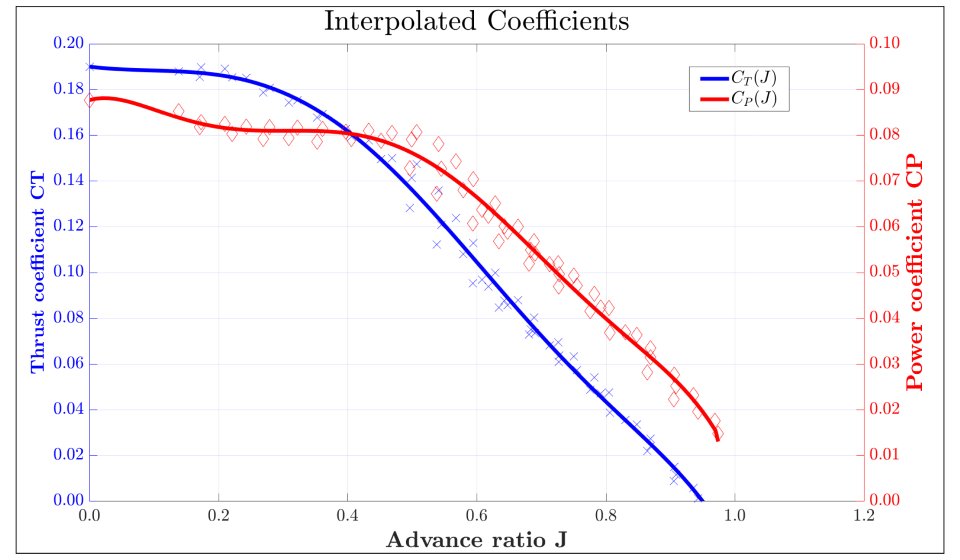
\includegraphics[width=0.5\textwidth]{graphs/coeffs-plot}
\vspace{-20pt}
\caption{Power \& thrust coefficients}
\label{fig:coeffs-plot}
\end{wrapfigure}
\par
Where $\Omega$ is the propellers rotational speed in [RPS] and $D$ is the propellers diameter in [mm]. For fixed pitch propellers the thrust and power coefficients are easily determined and remain consistent. Eq:\ref{eq:thrust-coefficient} and Eq:\ref{eq:power-coefficient} both vary due to what is defined as the \emph{advance ratio} $J$.
\begin{equation}\label{eq:advance}
J = \frac{v_\infty}{\Omega R}
\end{equation}
In most cases, the net head stream velocity $v_\infty$ is the perpendicular component (projected onto the plane's normal vector $\hat{n}$, Eq:\ref{eq:normal-fluid}) of the vehicles transnational velocity in the body frame, $\vec{v}_b\cdot\hat{n}$. For the case of a zero advance ratio, $J=0$, the conditions are regarded as static. Static thrust and power coefficients are nominal in their values. 
\end{minipage}
\par
\vspace{15pt}
Propeller databases like \cite{UIUC}\footnote{The UIUC database also includes blade profiles, pitch and chord lengths. The database is the outcome of \cite{lowreynolds}.} provide comprehensive values for a range of propeller types at different advance ratios. The introduction of those coefficients greatly simplifies the thrust estimation process. For a typical 6X4.5 inch propeller\footnote{Coefficients are linearly interpolated from similar pitched database results to match physical test values.}, the static thrust and power coefficients respectively are:
\begin{subequations}
\begin{equation}
{\color{blue}C_{T0}}=0.191
\end{equation}
\vspace{-20pt}
\begin{equation}
{\color{red}C_{P0}}=0.0877
\end{equation}
\end{subequations}
Fig:\ref{fig:coeffs-plot} shows the thrust, {\color{Blue}$C_{T}$}, and power, {\color{Red}$C_{P}$}, coefficients as a function of the advance ratio $J$. As the incident head fluid velocity, $v_\infty$, increases, the thrust coefficient decreases. So too does the power coefficient and hence the aerodynamic torque. The thrust and power coefficients can be assumed constant for low advance ratios, or in the case considered here, translational velocities.
\par
In Fig:\ref{fig:propeller-plots}, the thrust \& torque test rigs and the results of both static (thrust and torque) tests are plotted. In each test the measured values are shown ({\color{Red}$T(\Omega)$} \& {\color{Red}$Q(\Omega)$} with quadratic trend-lines) and an estimated value dependent on static coefficients ({\color{LimeGreen}$\hat{T}C_t(\Omega)$} \& {\color{LimeGreen}$\hat{Q}C_p(\Omega)$}). Using the results from the plot(s) in Fig:\ref{fig:coeffs-plot} as a lookup table and calculating the values from Eq:\ref{eq:coefficients}, induced propeller thrust and torques can be accurately modeled (\emph{quadratically}\footnote{The power term is cubic W.R.T its rotational velocity}). 
\par
Instantaneous advance ratios, or rather the propeller incident fluid flow(s), are dependent on the vehicle's net transnational and angular velocity. Such that the fluid velocity's normal component to the propeller plane is given by:
\begin{equation}\label{eq:normal-fluid}
v_\infty = (\vec{v}_b + \vec{L}_{arm}\times \vec{\omega}_b)\cdot \hat{n}
\end{equation}
Where $\vec{v}_b$ is the body's transnational velocity and $\vec{\omega}_b$ is the body's angular velocity, both transformed to the propeller's frame, $\in\mathcal{F}^{M_i}$. Furthermore $\hat{n}(\lambda_i,\alpha_i)$ is the unit vector normal to the propeller's rotational plane, dependent on the propeller's orientation relative to the body velocity. Then $J$ is calculated as in Eq:\ref{eq:advance}.
\begin{figure}[htbp]
\begin{subfigure}{0.5\textwidth}
\centering
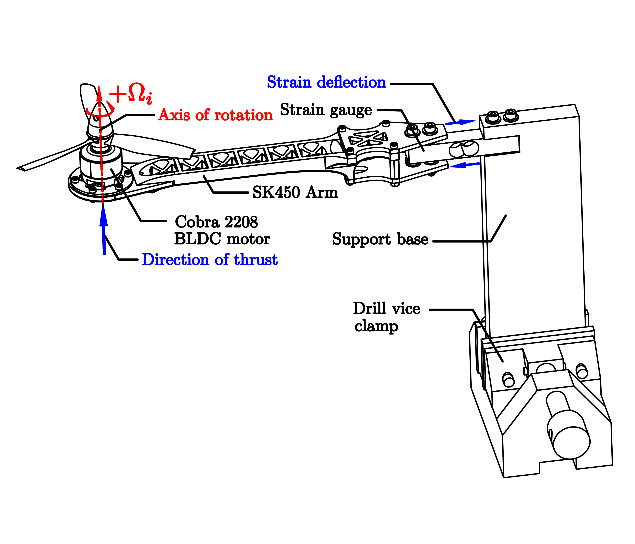
\includegraphics[width=\textwidth]{figs/thrust-rig}
\caption{Thrust test rig}
\label{fig:thrust-rig}
\end{subfigure}
\begin{subfigure}{0.5\textwidth}
\centering
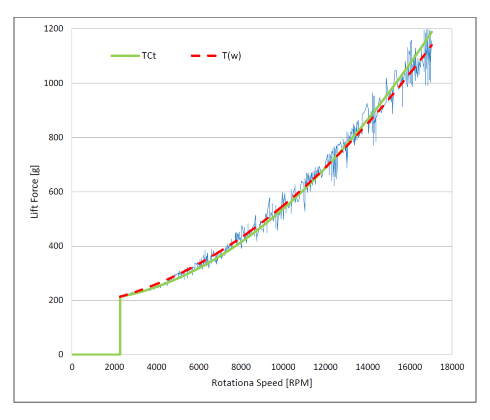
\includegraphics[width=\textwidth]{graphs/thrust-plot}
\caption{Thrust plot}
\label{fig:thrust-plot}
\end{subfigure}
\\
\begin{subfigure}{0.5\textwidth}
\centering
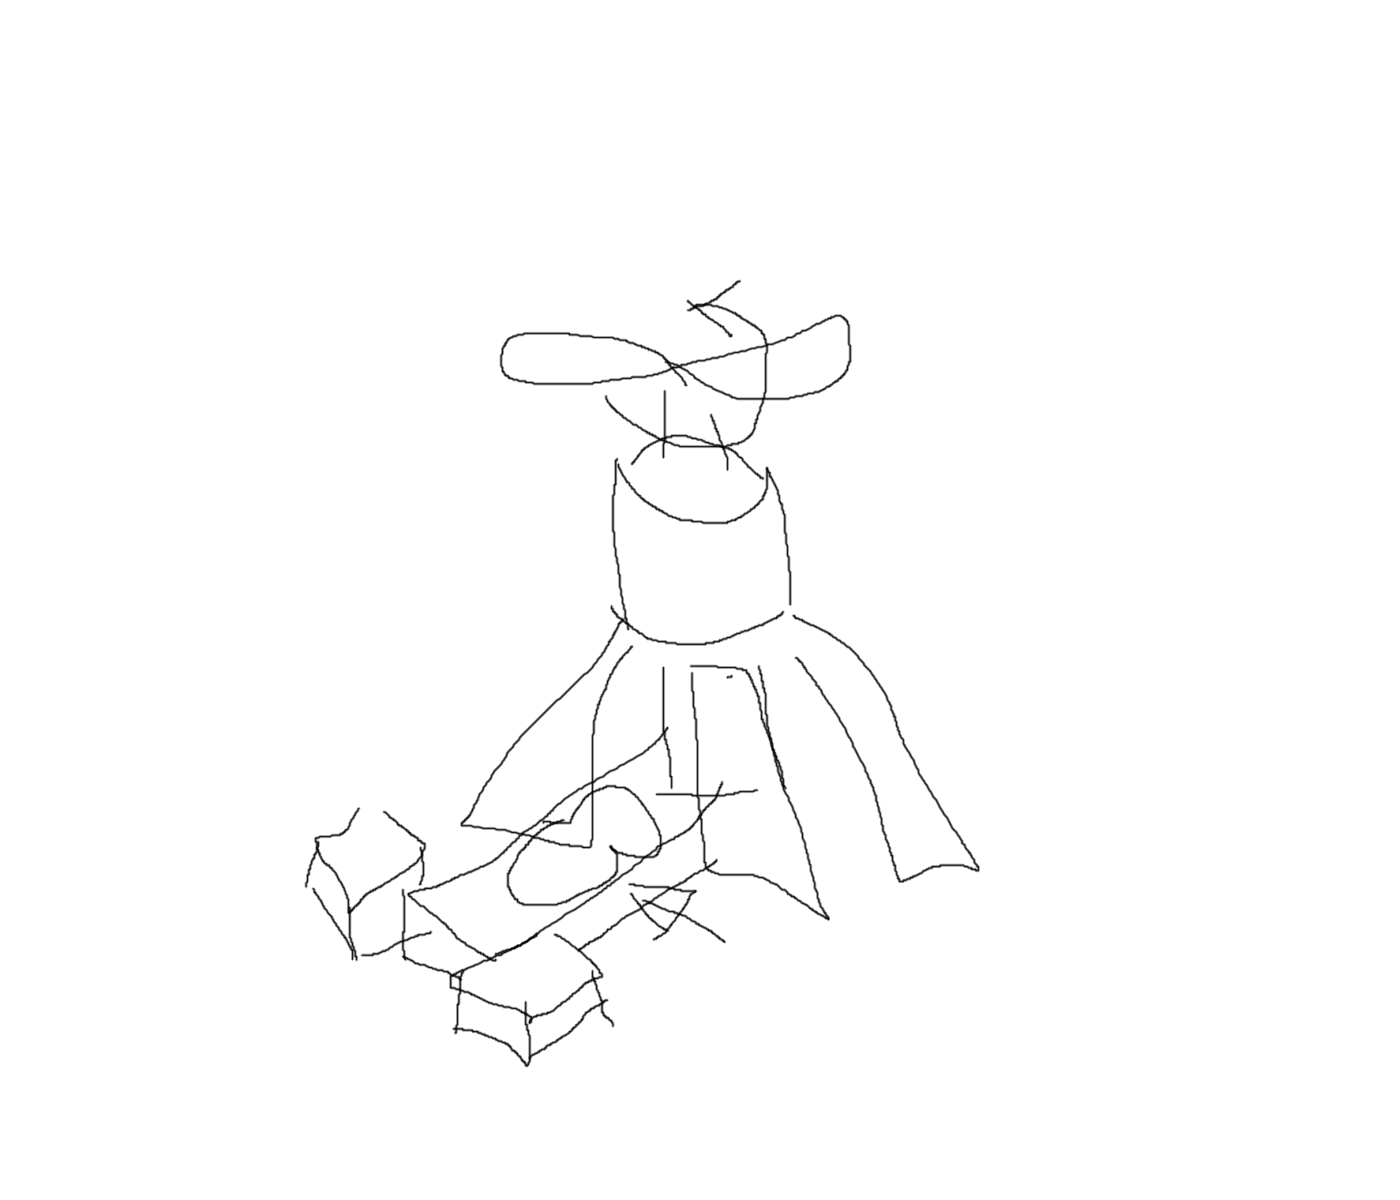
\includegraphics[width=\textwidth]{figs/torque-rig}
\caption{Torque test rig}
\label{fig:torque-rig}
\end{subfigure}
\begin{subfigure}{0.5\textwidth}
\centering
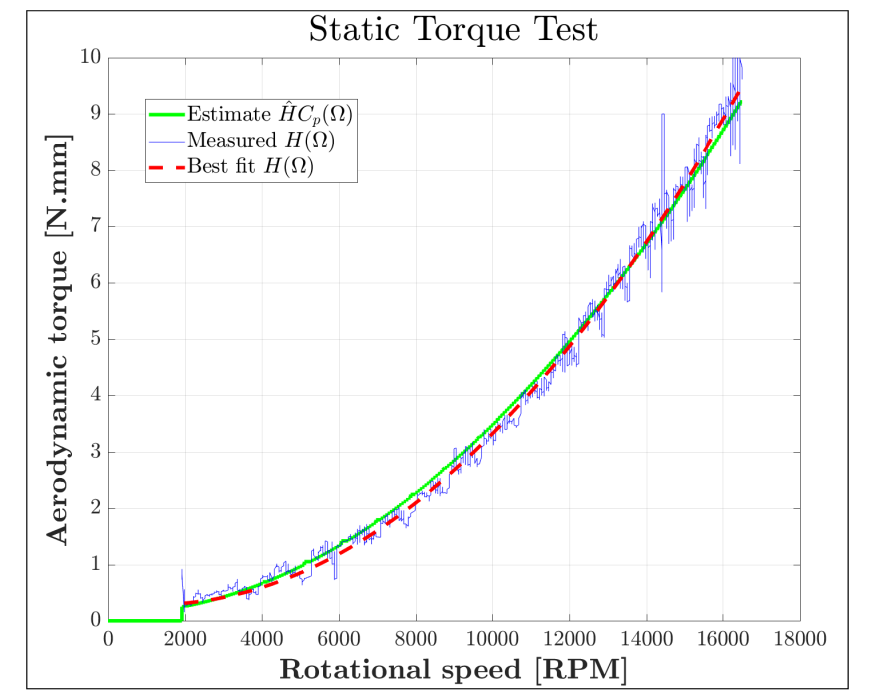
\includegraphics[width=\textwidth]{graphs/torque-plot}
\caption{Torque plot}
\label{fig:torque-plot}
\end{subfigure}
\caption{Static propeller tests}
\label{fig:propeller-plots}
\vspace{-20pt}
\end{figure}
\par
Counterclockwise and clockwise propellers and rotations were used for both thrust and torque tests. Despite the thrust and test rigs having been designed to isolate each respective response, the use of both directs allowed for opposing effects to cancel one another out. In the case of thrust tests plotted in Fig:\ref{fig:thrust-plot}; the opposing results were constructively averaged such that cross-directional torque effects on the strain gauge were cancelled out. 
\par
{\color{Gray}\emph{It's worth noting that the above static coefficients are indeed calculated from physical static tests. However advance ratio coefficient dependencies are linearly interpolated from the closest available matching data (APC Thin-Electric 8X6 propellers) cited from \cite{UIUC}}.}
\par
Conversely the recorded torque results, plotted in Fig:\ref{fig:torque-plot}, were subtractively averaged so that any erroneous perpendicular thrust deflection on the strain gauge was removed from the torque measurement. Both positive and negative rotational results for thrust and torque measurements are included in Appendix:\ref{app:thrust-torque}.
\par
{\color{Gray}\emph{Discrepancies which emerge between the model or coefficient values derived can be accounted for with lumped uncertainty disturbance term(s). Model uncertainty compensation can easily be incorporated into adaptive backstepping or $H_\infty$ control algorithms. The deviation of the modeled thrust or torques from their true values would be simple to incorporate into a plant dependent Lyapunov candidate function; Sec:\ref{subsubsec:control.attitude.nonlinear.adaptivebackstep}.}}
%====================================================
\subsection{Hinged Propeller Conning \& Flapping}
\label{subsec:dynamics.aero.flap}
%====================================================
Other non-linear effects which adversly effect a propeller's performance have all been well documented in the helicopter aerodynamic and propeller fields\cite{basichelicopter,bramwell}. Typically such affects are more pronounced when observing hinged variable pitch \footnote{Twisted, fixed pitched propellers are used on the prototype here and as such effects detailed in Sec:\ref{subsec:dynamics.aero.flap} are diminished. Moreover, low translational velocities suppress such responses but they're worth mentioning.} propellers. Conning and flapping are the two most significant aerodynamic responses produced by a propeller. Other phenomenon like cyclic vortex ring states aren't applicable here and fall outside the scope of the investigation. 
\par
\begin{figure}[htbp]
\centering
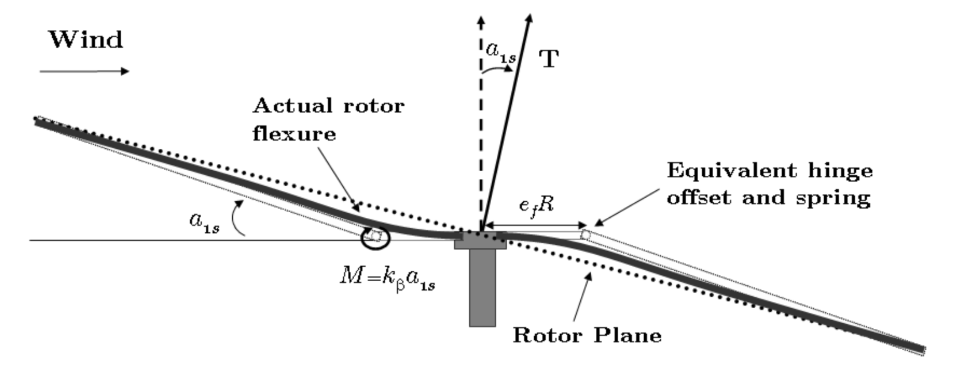
\includegraphics[width=0.95\textwidth]{figs/prop-flap}
\caption{Propeller blade flapping}
\label{fig:prop-flap}
\end{figure}
In translational flight for an unducted propeller each blade encounters varying incident fluid flow. The advancing blade, relative to the body's translational direction, encounters a greater fluid flow than the retreating blade. The result is that the effective local angle(s) of attack for the opposing advancing and retreating propeller blades aren't symmetrical. The unbalanced angles of attack produce a dissymmetry of lift across the propeller's surface.
\par
Throughout each rotation the blade is forced up and down as it cycles through varying fluid flows, applying a torque about the propeller's hub. The extent of that torque is dependent on the body's net translational velocity and the propeller material's suceptibility to deflection. The flapping pitches the effective propeller plane (\emph{tip-path plane}), and hence the thrust vector line, away from its principle axis, Fig:\ref{fig:prop-flap}\footnote{Diagram adapted from Hoffman et al.(2007)\cite{starmac}}.
\par
The overall net effect is that the propeller's thrust vector is pitched marginally away from an ideal perpendicular vector by some deflection angle. The phenomenon is diminished at low translational velocities and as such, isn't applicable to the range of flight envelopes which the prototype for this project will experience.
\par
\begin{figure}[hbtp]
\centering
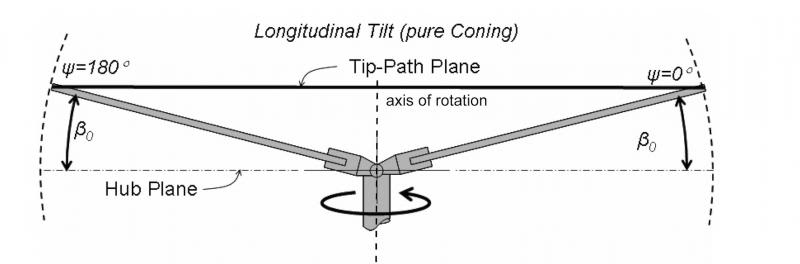
\includegraphics[width=0.95\textwidth]{figs/prop-coning}
\caption{Propeller coning}
\label{fig:prop-coning}
\end{figure}
Coning (illustrated in Fig:\ref{fig:prop-coning}) is another form of propeller deflection, which is again dependent on the blades stiffness properties, causes the propeller blades (advancing and retreating) to both deflect upward. Loading on the propeller surface and supporting a body's weight causes the upward deflection. The coning reduces the effective propeller disc's radius, adversely affecting thrust produced, Eq:\ref{eq:bem-thrust}. Increased loading accentuates the coning angle experienced by the propellers and as such alters the tip-path-plane.
\par
Both aerodynamic induced propeller deflection effects can be quantified numerically. Their derivation and resultant equations are cumbersome however. In due course their effect on the produced prototype which this project investigates isn't significant enough to produce instability if neglected. The frame could potentially be affected in more adverse ways given certain flight conditions with higher translational velocities or incident wind \& fluid flow disturbances\ldots
%====================================================
\subsection{Drag}
\label{subsec:dynamics.aero.drag}
%====================================================
For any solid body with some translational velocity motion within a fluid, there is a first order damping response opposing translational velocity. The net drag force, $\vec{D}_{net}$, although locally dependent on individual component cross-sections can be abstracted to a drag coefficient matrix representing the whole body.
\begin{equation}\label{eq:distrubance}
\vec{D}_{net}(\vec{v})=\begin{bmatrix}
A_{xx} & A_{xy} & A_{xz}\\
B_{yx} & B_{yy} & A_{yz}\\
C_{zx} & C_{zy} & C_{zz}
\end{bmatrix}
\begin{bmatrix}
u\\
v\\
w
\end{bmatrix}
~~~~\in\mathcal{F}^b
\end{equation}
\par
The drag coefficients, $A,B~\&~C$, are determined by the frames directional cross-section areas for each $\hat{X}_b,\hat{Y}_b,\hat{Z}_b$ axis. Given a well designed \& symmetrical frame, it can be assumed the off-diagonal elements aren't of consequence and as such the drag equation can be simplified to:
\begin{equation}
\vec{D}_{net}(\vec{v})\approx diag\big(A_{xx}~B_{yy}~C_{zz}\big)\vec{v}~~~~\in\mathcal{F}^b
\end{equation}
Without access to wind tunnel test facilities, the drag coefficients are difficult to empirically ascertain with a relative degree of certainty. As such the drag effects are relegated to the lumped disturbance \& uncertainty term(s) to be adpatively compensated for, Sec:\ref{subsubsec:control.attitude.nonlinear.adaptivebackstep}. Analogous drag-like opposing effects to angular rotation rates do exist but, for the intents and purposes of most practical flight envelopes, can be disregarded.
\par
In simulation; if the plant has sufficient disturbance rejection then a first order drag term in Eq:\ref{eq:distrubance} would be easily accounted for by the adaptive backstepping algorithm. It would be easy to physically test for the disturbance coefficients given further investigation on the prototype frame but, given the flight envelope for this research, is outside the scope of investigation here\ldots
%====================================================
\section{Consolidated Model}
\label{sec:dynamics.model}
%====================================================
Reiterating the different aspects detailed above and consolidating the state equations from Eq:\ref{eq:states.a}-\ref{eq:states.d}. Then lifting the attitude states to $\mathbb{R}^4$ space with the use of quaternions. Also introducing the non-linear inertial \& gyroscopic responses to induced perturbations, $\vec{\tau}_\lambda$ and $\vec{\tau}_\alpha$ from Eq:\ref{eq:torque-induced-inner} \& Eq:\ref{eq:torque-induced-middle} respectively, with non-linear inertial matrix terms $\mathbb{I}_b(u)$ from Section:\ref{sec:proto.inertia}. Finally replacing net \emph{virtual} plant inputs\footnote{Exact actuator relationships are explored in Section:\ref{sec:control.inputs}}, $\mu \vec{\tau}$ and $\mu \vec{F}$, with higher fidelity thrust models; produces the following set of state differentials used for control plant development \ldots
\\
\begin{subequations}\label{eq:quaternion-states}
\begin{equation}\label{eq:quaternion-states-velocity}
\dot{\mathcal{E}}=Q_b\otimes^*\vec{v}_b\otimes Q_b~~~~\in\mathcal{F}^I
\end{equation}
\vspace{-10pt}
\begin{equation}\label{eq:quaternion-states-acceleration}
\dot{\vec{v}}_b=m^{-1}\big(-\vec{\omega}_b\times m\vec{v}_b+Q_b\otimes m\vec{G}_I\otimes Q_b^*-\vec{D}_{net}(\vec{v}_b)+\mu\vec{F}(u)\big)~~~~\in\mathcal{F}^b
\end{equation}
\vspace{-8pt}
\begin{equation}\label{eq:quaternion-states-quaternion}
\dot{Q}_b=\frac{1}{2}Q_b\otimes \vec{\omega}_b ~~~~\in\mathcal{F}^I
\end{equation}
\vspace{-8pt}
\begin{equation}\label{eq:quaternion-states-angular}
\dot{\vec{\omega}}_b=\mathbb{I}_b(u)^{-1}\big(-\vec{\omega}_b \times \mathbb{I}_b(u)\vec{\omega}_b+\vec{\tau}_Q(u)+\vec{\tau}_g(u)+\sum \vec{Q}(\Omega,\lambda,\alpha)+\mu\vec{\tau}(u)\big)~~~~\in\mathcal{F}^b
\end{equation}
\vspace{-10pt}
\begin{equation}
u=\big[\Omega_1^+,~\lambda_1,~\alpha_1,~\ldots~\Omega_4^-,~\lambda_4,~\alpha_4 \big]~\in\mathbb{U}
\end{equation}
\end{subequations}
With net thrust and torque plant control inputs, $\mu\vec{F}$ \& $\mu\vec{\tau}$ respectively. Both are later abstracted to virtual control inputs next in Chapter:\ref{ch:control}, (\emph{individual motor number subscripts, $i\in[1:4]$, are implied}).
\begin{subequations}\label{eq:quaternion-inputs}
\begin{equation}
\mu\vec{F}(u)=\sum \vec{T}(\Omega,\lambda,\alpha)=\sum Q_{M_i}^*\otimes T(\Omega)\otimes Q_{M_i}~~~~\in\mathcal{F}^b
\end{equation}
\vspace{-6pt}
\begin{equation}
\mu\vec{\tau}(u)=\sum \vec{l}\times\vec{T}(\Omega,\lambda,\alpha)=\sum \vec{l}\times\big(Q_{M_i}^*\otimes T(\Omega)\otimes Q_{M_i}\big)~~~~\in\mathcal{F}^b
\end{equation}
\end{subequations}
The scalar thrust $T(\Omega)$ is a function of the propellers rotational velocity however $\vec{T}(\Omega,\lambda,\alpha)$ is a 3 dimensional thrust vector, redirected in the analogue of Eq:\ref{eq:motor-module-rotation.a} and transformed to the body frame $\mathcal{F}^b$. Equivalently $Q(\Omega)$\footnote{Disambiguation: $Q(\Omega)$ here is a torque, not a quaternion.} is the scalar aerodynamic torque term in $\mathcal{F}^{M_i}$ about each motor's rotor $\hat{Z}$-axis, $\vec{Q}(\Omega,\lambda,\alpha)$ is the torque vector counterpart in $\mathcal{F}^b$. Both thrust and aerodynamic propeller torque\footnote{Torque dependent on the power term calculated from Eq:\ref{eq:element-power}} terms are calculated from their respective coefficients (plotted in Fig:\ref{fig:coeffs-plot}):
\begin{subequations}
\begin{equation}\label{eq:aerodynamic-thrust}
T(\Omega)= C_T(J)\rho\Omega^2D^4
\end{equation}
\vspace{-15pt}
\begin{equation}\label{eq:aerodynamic-torque}
Q(\Omega)= C_P(J)\rho\Omega^3D^5 \frac{1}{R\Omega}
\end{equation}
\end{subequations}
Inertial torque responses from actuator input rates (\emph{in feedback\footnote{Response terms are used later as secondary actuator inputs in feedforward configuration rather than feedback terms to be compensated for.} configuration here}) from Eq:\ref{eq:torque-response};
\begin{equation}\label{eq:actuator-torque}
\tau_Q(u)=\sum_{i=1}^4 -Q_{M_i}\otimes \tau_{\lambda_i}(u)\otimes Q_{M_i}^*-Q_{M_i'}\otimes \tau_{\alpha_i}(u) \otimes Q_{M_i'}^*~~~\in\mathcal{F}^b
\end{equation}
And the variable gravitational torque arm from Eq:\ref{eq:grav-torque}, dependent on net actuator positions $u$:
\begin{equation}\label{eq:grav-torque}
\vec{\tau}_g(u)=\Delta C.G \times\vec{G}_b
\end{equation}
Finally, the body's net inertial tensor, taken from Eq:\ref{eq:body-net} is given as:
\begin{equation}
\underset{u\in\mathbb{U}}{\mathbb{I}_b(u)}=\mathbb{I}_{body}+\sum_{i=1}^{4} \mathbb{M}_{inner}+\sum_{i=1}^{4} \mathbb{M}_{middle}
\end{equation}
It is possible to bundle both attitude states (either euler angles $\vec{\eta}$ or quaternions $Q_b$) together with the linear translational position $\mathcal{E}$ into a single state vector $\mathbf{x}$. Which then has its own combined control law. This could potentially exploit the cross-product coupling terms between angular and linear displacements for control benefits.